%=====================================================
% PREÂMBULO - CONFIGURAÇÕES GERAIS DO DOCUMENTO
%======================================================
\documentclass[12pt, a4paper, openright, oneside, brazilian]{abntex2}

% --- PACOTES DE CODIFICAÇÃO ---
\usepackage{fontenc}
\usepackage[utf8]{inputenc}

% --- PACOTES DE LAYOUT E FORMATAÇÃO (ABNT/UNESP) ---
\usepackage[left=3cm, top=3cm, right=2cm, bottom=2cm, headsep=1.5cm]{geometry}
\usepackage{indentfirst} % Indenta o primeiro parágrafo de cada seção
% Usando o comando nativo da classe memoir (base do abntex2) para espaçamento 1,5 [1]
\OnehalfSpacing
% --- PACOTES DE BIBLIOGRAFIA (ABNT) ---
\usepackage{csquotes}
% Opções simplificadas para máxima compatibilidade.
\usepackage[backend=biber, style=abnt]{biblatex}
\addbibresource{bibliografia.bib} % Seu arquivo.bib

% --- PACOTES MATEMÁTICOS ---
\usepackage{amsmath}
\usepackage{amssymb}
\usepackage{mathtools}

% --- PACOTES PARA TABELAS E FIGURAS ---
\usepackage{graphicx}
\usepackage{booktabs}
\usepackage{multirow}
\usepackage{array}
\usepackage[table]{xcolor}
\usepackage{caption}
\usepackage{float}
\captionsetup{
    format=plain,
    justification=justified,
    singlelinecheck=false,
    font=small,
    labelfont=bf,
    labelsep=period
}

% --- PACOTES ADICIONAIS ---
\usepackage{ragged2e}
\usepackage{soul}

% --- CONFIGURAÇÃO DE HIPERLINKS ---
\hypersetup{
    colorlinks=true,
    linkcolor=blue,
    citecolor=green!50!black,
    urlcolor=blue!80!black,
    pdftitle={Desenvolvimento e Análise de um Controlador Eletrônico de Velocidade para Motores de Corrente Contínua Sem Escovas},
    pdfauthor={Enzo Luiz Fernandes},
    bookmarksopen=true
}

%=====================================================
% METADADOS DO TRABALHO (PARA CAPA E FOLHA DE ROSTO AUTOMÁTICAS)
%=====================================================

\titulo{Desenvolvimento e Análise de um Controlador Eletrônico de Velocidade para Motores de Corrente Contínua Sem Escovas}
\autor{Enzo Luiz Fernandes}
\instituicao{
  Universidade Estadual Paulista "Júlio de Mesquita Filho"
  \par
  Faculdade de Engenharia de Ilha Solteira
  \par
  Departamento de Engenharia Elétrica
}
\local{Ilha Solteira}
\data{2025}
\tipotrabalho{Trabalho de Conclusão de Curso}
\orientador{Prof. Dr. Guilherme de Azevedo e Melo}
\tipotrabalho{monografia}
\preambulo{Trabalho de Conclusão de Curso apresentado ao Departamento de Engenharia Elétrica da Faculdade de Engenharia de Ilha Solteira, da Universidade Estadual Paulista "Júlio de Mesquita Filho", como parte dos requisitos para obtenção do título de Bacharel em Engenharia Elétrica.}

\begin{document}

% --- ELEMENTOS PRÉ-TEXTUAIS --
\begin{center}

\includegraphics[width=9cm]{imagens/logoUNESP.jpg} 
\end{center}

\vspace{1.5cm} 
\imprimircapa
%\imprimirfolhaderosto

% Folha de Aprovação
\begin{folhadeaprovacao} 
\begin{center}
{\ABNTEXchapterfont\large\textsc{\imprimirautor}}
\par\vspace{\onelineskip}
{\ABNTEXchapterfont\Large\bfseries\imprimirtitulo} 
\end{center} 
\vspace{1cm} 
\hspace{.45\textwidth} \begin{minipage}{.5\textwidth} 
\imprimirpreambulo 
\end{minipage} 
\vspace{1cm}
\par\vspace{\onelineskip}
Trabalho aprovado. \imprimirlocal, \imprimirdata: 

%Assinaturas 
\assinatura{\imprimirorientador \\UNESP} 
\assinatura{Assinatura 2\\ UNESP} 
\assinatura{Assinatura 3 \\ UNESP} 

\begin{center} 
\vfill 
{\large\imprimirlocal} 
\par 
{\large\imprimirdata} 
\end{center} 
\end{folhadeaprovacao}

% RESUMO E ABSTRACT
\begin{abstract}
    Este trabalho aborda o desenvolvimento e a análise de um controlador eletrônico de velocidade (ESC) para motores de corrente contínua sem escovas (BLDC). A investigação inicia com uma robusta fundamentação teórica sobre os princípios de funcionamento, construção e os parâmetros chave dos motores BLDC, como as constantes de torque ($K_T$) e de velocidade ($K_V$), cuja equivalência intrínseca é demonstrada por meio de um balanço de potência. Em seguida, são detalhados os algoritmos de controle, com foco na comutação de seis passos e na modulação por largura de pulso (PWM). A metodologia do projeto é delineada em três fases: simulação computacional para validação do conceito, projeto do circuito eletrônico com seleção criteriosa de componentes incluindo o microcontrolador ESP32 e uma bateria LiPo dimensionada para a aplicação e, por fim, a prototipagem e testes experimentais para verificar o desempenho do controlador. O objetivo é produzir um protótipo funcional que ofereça uma operação suave e precisa, validando os conceitos teóricos e as escolhas de projeto.
    \par\vspace{\onelineskip} % Espaço antes das palavras-chave
    \noindent\textbf{Palavras-chave:} Motor BLDC. Controlador Eletrônico de Velocidade. Controle de Motores. ESP32.
\end{abstract}

\begin{abstract} 
\begin{otherlanguage*}{english}
This work addresses the development and analysis of an electronic speed controller (ESC) for brushless direct current (BLDC) motors. The investigation begins with a robust theoretical foundation on the operating principles, construction, and key parameters of BLDC motors, such as the torque ($K_T$) and velocity ($K_V$) constants, whose intrinsic equivalence is demonstrated through a power balance analysis. Subsequently, control algorithms are detailed, focusing on six-step commutation and pulse-width modulation (PWM). The project methodology is outlined in three phases: computational simulation for concept validation, electronic circuit design with careful selection of components—including the ESP32 microcontroller and a LiPo battery sized for the application—and finally, prototyping and experimental testing to verify the controller's performance. The objective is to produce a functional prototype that offers smooth and precise operation, validating the theoretical concepts and design choices.
    \par\vspace{\onelineskip}
    \noindent\textbf{Keywords:} BLDC Motor. Electronic Speed Controller. Motor Control. ESP32.
\end{otherlanguage*}
\end{abstract}

% LISTAS E SUMÁRIO

\newpage
\pdfbookmark{\listfigurename}{lof}
\listoffigures*
\cleardoublepage

\pdfbookmark{\listtablename}{lot}
\listoftables*
\cleardoublepage

\pdfbookmark{\contentsname}{toc}
\tableofcontents*
\cleardoublepage

% --- ELEMENTOS TEXTUAIS ---
\textual

\chapter{Introdução Teórica}

Os motores BLDC (\textit{Brushless Direct Current Motor}) representam um avanço significativo em relação aos motores CC tradicionais porque eliminam a necessidade de escovas mecânicas para a conversão de energia, resultando em maior rendimento energético, menos desgaste e maior vida útil \cite{hanselman2003brushless}. Esses avanços tecnológicos estão sendo impulsionados pela crescente demanda por sistemas de acionamento mais eficientes, confiáveis e de baixa manutenção em diversas aplicações industriais, comerciais e de consumo. A precisão e controlabilidade dos motores BLDC os tornam ideais para aplicações que exigem alta exatidão de movimento, velocidade e controle de torque, como robótica, automação industrial, veículos elétricos e eletrônicos de consumo.

\section{Motores CC Sem Escova}
O princípio de funcionamento dos motores BLDC é baseado em campos magnéticos gerados por ímãs permanentes e enrolamentos de  (Figura \ref{Configuração de um motor DC convencional (A) e motor BLDC (B).}). A comutação da corrente para gerar movimento ocorre eletronicamente, por meio de um controlador dedicado normalmente chamado de ESC (Eletronic Speed Controller), que pode usar ou não sensores durante o processo, eliminando assim a necessidade de escovas mecânicas utilizadas em motores DC tradicionais. Esta abordagem resulta em uma diminuição significativa do desgaste mecânico, aumentando a vida útil do motor e reduzindo a necessidade de manutenção.

\begin{figure}[h]
	\centering
	\caption{Configuração de um motor DC convencional (A) e motor BLDC (B).}
	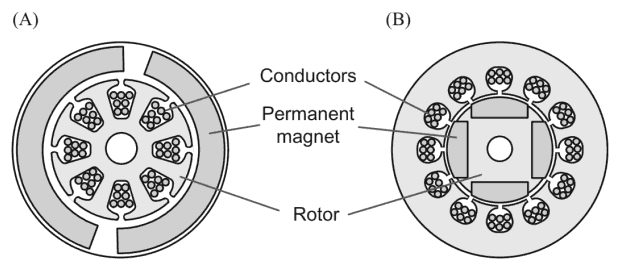
\includegraphics[width=8cm]{imagens/Comparativo.png}
	\caption*{Fonte:\cite{kim2017electric}.}
 \label{Configuração de um motor DC convencional (A) e motor BLDC (B).}
\end{figure}

Amplamente utilizados em uma variedade de aplicações, desde eletrônicos de consumo, como ventiladores e ferramentas elétricas, até aplicações industriais e automotivas. Sua capacidade de fornecer um controle preciso de velocidade e posição, juntamente com uma resposta rápida, faz deles a escolha ideal para sistemas que exigem rendimento energético e alta performance.

Apesar das muitas vantagens, não estão isentos de algumas limitações. A complexidade eletrônica necessária para o controle preciso, o custo inicial potencialmente mais elevado comparado a motores elétricos escovados, a sensibilidade a ambientes de alta temperatura, pois podem gerar a desmagnetização dos imãs permanentes, a exigência de eletrônica de controle especializada, o potencial de ruído eletromagnético (EMI) e a complexidade de manutenção do sistema como um todo são fatores a serem considerados ao escolher essa tecnologia. Cada aplicação específica deve ponderar essas considerações em relação aos benefícios que os BLDC oferecem, como rendimento, durabilidade e controle superior.

São categorizados como síncronos, ou seja, o rotor gira na mesma frequência do campo magnético gerado pelo estator \cite{jahns1984torque}. Também não apresentam o fenômeno de escorregamento que é característico dos motores de indução. Os motores BLDC estão disponíveis em configurações de uma fase, duas fases e três fases, sendo  essa a mais amplamente utilizada, por serem equilibrados em relação a oscilação de torque e custo de construção \cite{hendershot1994design}.

A nomenclatura "Brushless DC" pode gerar uma interpretação equivocada. Embora alimentado por uma fonte de corrente contínua (DC), o motor BLDC é, em sua essência, um motor síncrono de ímãs permanentes (PMSM) \parencite{maquinasEletricasFitzgerald}. A rotação é induzida por campos magnéticos girantes gerados nos enrolamentos do estator, que são alimentados por formas de onda de corrente alternada (AC) sintetizadas por um controlador eletrônico. Portanto, a designação "DC" refere-se à fonte de alimentação externa, e não ao princípio físico de operação interna, que requer uma lógica de controle sofisticada para operar \parencite{ti2013sensorless}.

Nesse contexto, a performance do sistema é governada por parâmetros intrínsecos que descrevem a física da conversão de energia. Duas das mais importantes dessas constantes são a \textbf{constante de torque ($K_T$)} e a \textbf{constante de velocidade ($K_V$)}. Estes parâmetros são a manifestação matemática dos princípios físicos que regem a interação entre os domínios elétrico e mecânico do motor.

\subsection{Fundamentos Físicos da Conversão Eletromecânica}

A operação de um motor elétrico é governada por dois princípios físicos interligados: a Força de Lorentz, que gera o torque, e a Lei da Indução de Faraday, que gera uma força contraeletromotriz.

\subsubsection{A Força de Lorentz}

A produção de força mecânica em um motor origina-se na Força de Lorentz. Esta lei descreve a força ($F$) sobre um condutor de comprimento ($L$) percorrido por uma corrente ($I$) e imerso em um campo magnético de densidade de fluxo ($B$). A relação vetorial é:
\begin{equation}
    F = I(L \times B)
\end{equation}
Em um motor rotativo, quando uma corrente flui através dos condutores do enrolamento, cada um experimenta uma força de Lorentz. Como esses condutores estão a um raio ($r$) do eixo de rotação, essa força linear se traduz em um torque eletromagnético ($T_e$), estabelecendo a ligação direta entre a entrada elétrica (corrente) e a saída mecânica (torque).

\subsubsection{A Lei de Faraday}
Simultaneamente à produção de torque, um motor em rotação atua como um gerador. A Lei da Indução de Faraday afirma que a variação do fluxo magnético através de uma espira de fio induz uma força eletromotriz (FEM). Em um motor, o movimento dos ímãs do rotor em relação aos enrolamentos do estator induz uma tensão conhecida como \textbf{força contraeletromotriz (FCEM)}, ou \textit{back-EMF}.

De acordo com a Lei de Lenz, a polaridade desta tensão induzida ($e_a$) se opõe diretamente à tensão terminal ($V$) aplicada ao motor \parencite{infineon2011bldc}. A magnitude da FCEM é diretamente proporcional à velocidade angular ($\omega$) do motor, estabelecendo a ligação física entre o movimento mecânico (velocidade) e um fenômeno elétrico (tensão induzida).

\subsection{Modelo Matemático do Motor e a Definição das Constantes}

Os princípios de Lorentz e Faraday são sintetizados em um modelo matemático que descreve a dinâmica do motor.

\textbf{Equação Elétrica (Lei de Kirchhoff):}
\begin{equation}
    V = e_a + I_a R_a + L_a \frac{dI_a}{dt}
\end{equation}
Onde $V$ é a tensão aplicada, $e_a$ é a FCEM, $I_a R_a$ é a queda de tensão resistiva e $L_a \frac{dI_a}{dt}$ é a queda de tensão indutiva \parencite{maquinasEletricasFitzgerald}.

\textbf{Equação Mecânica (2ª Lei de Newton para Rotação):}
\begin{equation}
    T_e = T_l + J \frac{d\omega}{dt} + B\omega
\end{equation}
Onde $T_e$ é o torque eletromagnético, $T_l$ é o torque de carga, $J\frac{d\omega}{dt}$ é o torque inercial e $B\omega$ é o torque de atrito viscoso \parencite{maquinasEletricasFitzgerald}.

Dentro deste modelo, as constantes do motor surgem como os fatores de proporcionalidade que conectam os domínios elétrico e mecânico.

\subsection{\texorpdfstring{A constante de Torque $K_T$}{A constante de Torque KT}}
\label{KT}
A constante de torque ($K_T$) define a capacidade de um motor de converter corrente elétrica em torque mecânico. É formalmente definida como a relação linear:
\begin{equation}
    T_e = K_T I_a
\end{equation}
O valor de $K_T$ não é arbitrário, mas determinado pelas características construtivas do motor \parencite{hendershot1994design}:
\begin{itemize}
    \item \textbf{Força do Campo Magnético ($B$):} Ímãs mais fortes (ex: Neodímio) resultam em um $K_T$ maior.
    \item \textbf{Configuração do Enrolamento:} É diretamente proporcional ao número de espiras ($N$) nos enrolamentos.
    \item \textbf{Geometria do Motor:} Dimensões como o comprimento e o raio do estator influenciam diretamente seu valor.
\end{itemize}
Para um dado torque de carga, um motor com $K_T$ maior demandará uma corrente menor, resultando em menores perdas por efeito Joule ($P = I^2 R$) e, portanto, maior eficiência.

\subsection{\texorpdfstring{As constantes de Velocidade $K_V$}{As constantes de Velocidade KV}}
\label{KV}

De forma análoga, a relação entre a FCEM e a velocidade é quantificada por constantes.
\begin{itemize}
    \item \textbf{Constante de FCEM ($K_e$):} É a constante física que relaciona a FCEM gerada ($e_a$) com a velocidade angular do motor ($\omega$):
    \begin{equation}
        e_a = K_e \omega
    \end{equation}
    Assim como $K_T$, $K_e$ (também denotado como $k_b$) depende do projeto físico do motor \parencite{zoltan2012understanding}.

    \item \textbf{Constante de Velocidade ($K_V$):} Muito mais comum em folhas de dados comerciais, $K_V$ é definida como a relação entre a velocidade do motor sem carga e a tensão aplicada, geralmente em unidades de \textbf{RPM/V}. A relação entre $K_V$ e $K_e$ é de simples inversão \parencite{infineon2011bldc}:
    \begin{equation}
        K_V = \frac{1}{K_e}
    \end{equation}
    A FCEM é o mecanismo que limita a velocidade máxima do motor. O motor acelera até que a FCEM ($e_a = K_e \omega$) se aproxime da tensão de alimentação ($V$), ponto no qual a corrente resultante é apenas suficiente para vencer o atrito.
\end{itemize}

\subsection{A Equivalência entre $K_T$ e $K_e$}

Um dos resultados mais notáveis na teoria de motores é a equivalência numérica entre $K_T$ e $K_e$ quando ambas são expressas em unidades do Sistema Internacional (SI): \textbf{Nm/A} para $K_T$ e \textbf{V·s/rad} para $K_e$.
\begin{equation}
    K_T \text{ [Nm/A]} = K_e \text{ [V·s/rad]}
\end{equation}
Esta equivalência não é uma coincidência, mas uma consequência da \textbf{lei da conservação de energia}.

\textbf{Demonstração por Balanço de Potência:}
\begin{enumerate}
    \item A potência elétrica convertida em potência mecânica ($P_{\text{conv}}$) é a parte da potência de entrada que não é perdida como calor nos enrolamentos.
    \[ P_{\text{conv}} = P_{\text{in}} - P_{\text{perdas}} = (V \cdot I_a) - (I_a^2 R_a) \]
    \item Usando a equação elétrica ($V = e_a + I_a R_a$), substituímos $V$:
    \[ P_{\text{conv}} = (e_a + I_a R_a)I_a - I_a^2 R_a = e_a I_a + I_a^2 R_a - I_a^2 R_a = e_a I_a \]
    \item A potência mecânica de saída ($P_{\text{mec}}$) é o produto do torque e da velocidade angular:
    \[ P_{\text{mec}} = T_e \omega \]
    \item Pela conservação de energia, $P_{\text{conv}} = P_{\text{mec}}$:
    \[ e_a I_a = T_e \omega \]
    \item Agora, substituímos as definições de $K_e$ e $K_T$ ($e_a = K_e \omega$ e $T_e = K_T I_a$):
    \[ (K_e \omega) I_a = (K_T I_a) \omega \]
    \item Para qualquer condição de operação não nula, podemos cancelar $\omega$ e $I_a$ de ambos os lados, provando que:
    \begin{equation}
        K_e = K_T
    \end{equation}
\end{enumerate}
Esta prova revela que o mesmo mecanismo de acoplamento eletromagnético que produz torque a partir da corrente (princípio motor, $K_T$) é o que gera tensão a partir do movimento (princípio gerador, $K_e$). Eles são duas manifestações do mesmo fenômeno físico \parencite{zoltan2012understanding, garcia1997modelagem}.

\subsection{Conversão de Unidades}

A elegância teórica é frequentemente obscurecida pelo uso de unidades inconsistentes na prática. A habilidade de converter valores de folhas de dados para o padrão SI é indispensável. A relação prática mais importante é entre $K_T$ e $K_V$:
\begin{equation}
    K_T \text{ [N·m/A]} \approx \frac{9.549}{K_V \text{ [RPM/V]}}
\end{equation}
Esta fórmula é derivada diretamente da equivalência $K_T = K_e = 1/K_V$ após a conversão de RPM para rad/s \parencite{infineon2011bldc}. A tabela abaixo resume as conversões chave.

\begin{table}[h!]
\centering
\caption{Unidades de Constantes de Motor e Fatores de Conversão para o SI}
\label{tab:unidades}

\resizebox{\columnwidth}{!}{

\begin{tabular}{llll}
\toprule
\textbf{Parâmetro} & \textbf{Unidade SI} & \textbf{Unidades Comuns Não-SI} & \textbf{Fórmula de Conversão para SI} \\
\midrule
\textbf{Constante de Torque ($K_T$)} & N·m/A & oz-in/A & 1 oz-in/A = 0.00706155 N·m/A \\
 & & mN·m/A & 1 mN·m/A = 0.001 N·m/A \\
\addlinespace
\textbf{Constante de FCEM ($K_e$)} & V·s/rad & V/krpm & 1 V/krpm = 0.009549 V·s/rad \\
\addlinespace
\textbf{Constante de Velocidade ($K_V$)} & rad/(V·s) & RPM/V & 1 RPM/V = 0.10472 rad/(V·s) \\
\bottomrule
\end{tabular}
}
\caption*{Fonte:Elaborado pelo autor.}
\end{table}

\subsection{A Constante do Motor ($K_m$) como Figura de Mérito}

Uma constante mais fundamental para avaliar a qualidade do projeto de um motor é a \textbf{constante do motor ($K_m$)}:
\begin{equation}
    K_m = \frac{K_T}{\sqrt{R_a}}
\end{equation}
Sua unidade no SI é \textbf{N·m/$\sqrt{\text{W}}$}. $K_m$ representa a capacidade do motor de produzir torque por watt de potência dissipada como calor. Um $K_m$ mais alto indica um motor mais eficiente na conversão de energia. Notavelmente, $K_m$ é invariante a alterações no enrolamento para um mesmo tamanho de carcaça, tornando-se uma excelente figura de mérito para comparar a qualidade de diferentes projetos de motores \parencite{infineon2011bldc}.

\subsection{Influência da Temperatura}

Embora chamadas de "constantes", $K_T$ e $K_e$ são afetadas pela temperatura. O aquecimento do motor causa uma redução na força magnética dos ímãs permanentes. Como ambas as constantes são diretamente proporcionais à densidade de fluxo magnético, um motor operando em alta temperatura produzirá menos torque para a mesma corrente (menor $K_T$) e precisará girar mais rápido para gerar a mesma FCEM (menor $K_e$, consequentemente um $K_V$ ligeiramente maior), resultando em uma performance geral degradada.

\section{Controlador Eletrônico de Velocidade (ESC)}
Os controladores eletrônicos de velocidade, são dispositivos eletrônicos que controlam a velocidade e o torque de motores BLDC. São classificados pela sua corrente e tensão máxima de saída. São constituídos dos seguintes componentes básicos:

\begin{itemize}
\item Circuito de entrada: O circuito de entrada converte a tensão fornecida pela bateria em tensão que pode ser usada pelo circuito de controle utilizando PWM para gerar uma tensão média desejada que será fornecida ao motor. Também pode inverter a sequência de comutação das fases fazendo com que o sentido de rotação também seja invertido.
\item Circuito de controle: O circuito de controle é responsável por calcular a corrente que deve ser fornecida às bobinas do motor. Normalmente se utilizam de sinais com características de PWM como sinal de referência para definir a velocidade e sentido de rotação.
\item Circuito de saída: O circuito de saída fornece a corrente necessária às bobinas do motor.
\end{itemize}

Além desses componentes básicos, os ESCs para motor BLDC pode incluir os seguintes recursos, além dos já discutidos anteriormente:

\begin{itemize}
\item Filtro de ruído: O filtro de ruído é usado para reduzir o ruído elétrico que pode ser gerado pelo motor.
\item Proteção térmica: A proteção térmica é usada para proteger o motor de superaquecimento.
\item Proteção contra sobrecarga: O ESC pode desligar o motor se ele experimentar correntes superiores às nominais que representam riscos de deterioração das bobinas do motor.
\end{itemize}

\subsection{O Papel do Controlador (ESC) e o Controle Vetorial (FOC)}

As equações lineares de um motor DC só são diretamente aplicáveis a um motor BLDC devido à ação sofisticada do seu \textbf{Controlador Eletrônico de Velocidade (ESC)}. O ESC realiza a comutação eletrônica, energizando sequencialmente os enrolamentos do estator para criar um campo magnético giratório.

A técnica de controle de ponta que aperfeiçoa essa analogia é o \textbf{Controle Vetorial (FOC)}. O FOC transforma matematicamente as correntes trifásicas em um referencial giratório (d-q), separando a corrente em um componente que produz fluxo ($I_d$) e outro que produz torque ($I_q$). Ao manter $I_d = 0$, o controlador faz com que o torque seja linearmente proporcional apenas a $I_q$. Isso força a complexa máquina AC a se comportar como o motor DC idealizado, tornando as constantes $K_T$ e $K_e$ ferramentas de análise e projeto perfeitamente válidas \parencite{hendershot1994design}.

\subsection{Consequências Práticas da Seleção de $K_V$}

A seleção de $K_V$ é uma decisão de projeto crítica que estabelece um compromisso fundamental:
\begin{itemize}
    \item \textbf{Motores de Alto $K_V$:} Possuem menos espiras de fio mais grosso. Resultam em baixo $K_T$, baixa resistência e baixa indutância. Para produzir torque, exigem alta corrente, mas atingem altas velocidades. Ideais para aplicações de alta velocidade e baixo torque, como drones de corrida e fusos de usinagem \parencite{tmotor2019kv}.
    \item \textbf{Motores de Baixo $K_V$:} Possuem mais espiras de fio mais fino. Resultam em alto $K_T$, alta resistência e alta indutância. Geram alto torque com baixas correntes, sendo mais eficientes para essa finalidade, mas com menor velocidade máxima. Ideais para aplicações de acionamento direto e alto torque, como drones de carga, guinchos e atuadores robóticos \parencite{byod2018kv}.
\end{itemize}

\subsection{Princípios de Operação}

 O controlador do motor deve fornecer corrente e tensão adequadas às bobinas do estator do motor, a fim de controlar a velocidade e o torque do motor \cite{jahns1996pulsating}. O circuito básico que realiza esse papel é o de uma ponte inversora trifásica, onde o motor BLDC pode estar conectado em Estrela ou Delta. O controle do circuito de disparo dos transistores do inversor deve ser feito de forma que cada fase do estator seja percorrida por uma corrente com a forma de onda senoidal ou trapezoidal, voltadas respectivamente para alto rendimento e baixo custo. As formas de onda de cada uma das fases devem estar defasadas entre si, permitindo que o motor gire de forma contínua.

\subsubsection{Comutação de Seis Passos}

A comutação de seis passos demanda um sincronismo de disparo dos transistores, de modo que sempre dois deles estejam fechados, formando um circuito tal que a cada $60 ^\circ$ elétricos o par de fases percorridas pela corrente se alterne (Figura \ref{Sequência de acionamento para um BLDC trifásico}). Cada transistor permanece em condução durante $120 ^\circ$ elétricos. Vale ressaltar que os eventos de condução e bloqueio, denominados comutações dos transistores, geram variações na corrente e isso é responsável pelas oscilações no torque do motor \cite{kim2017electric}. 

\begin{figure}[p]
	\centering
	\caption{Sequência de acionamento para um BLDC trifásico.}
	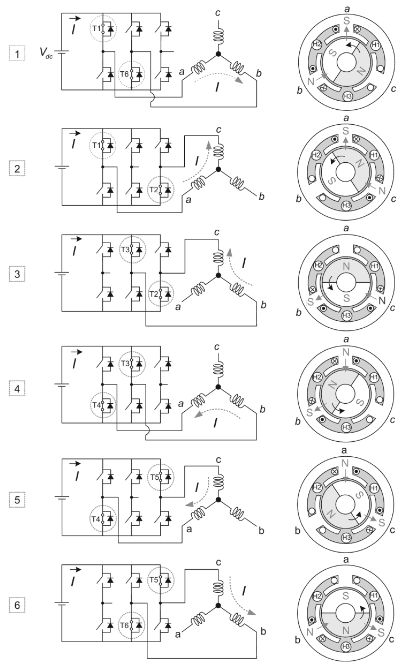
\includegraphics[width=10cm]{imagens/acionamento.png}
	\caption*{Fonte:\cite{kim2017electric}.}
 \label{Sequência de acionamento para um BLDC trifásico}
\end{figure}

Esse é o algoritmo de acionamento dos transistores mais amplamente utilizado para controlar motores BLDC e é também chamada de Controle Trapezoidal. Para se saber quando e quais deles acionar, existem duas opções, saber a posição que o rotor se encontra de forma a acionar o conjunto de transistores seguinte. Para esse tipo de controle se dá o nome de Controle de Malha Fechada. Também é possível acionar os indutores a partir de uma sequência fixa determinada pelo circuito, o que faz com que o rotor comece a girar em algum momento da sequência e siga girando a partir da sequência determinada. Esse tipo de controle é mais simples e de menor custo, porém não tão preciso, recebendo o nome de Controle de Malha Aberta.

 Para a realização do Controle de Malha Fechada é possível usar um sensor de efeito Hall capaz de identificar o campo magnético resultante da interação do campo eletromagnético das bobinas e do campo magnético dos imãs permanentes do rotor, indicando a seção que o campo eletromagnético resultante encontra-se, ou seja, sua posição angular. Partindo dessa referência, se pode saber quais transistores devem ser acionadas para que o rotor continue a girar. A utilização de sensor Hall também propicia a determinação da velocidade angular do motor. Esse método é mais complexo e de maior custo, porém garante uma maior confiabilidade em relação a velocidade.

Quando a aplicação necessita que o motor possua apenas uma velocidade, a fonte de alimentação de tensão fixa é suficiente, mas para casos onde é necessário varia a velocidade do motor precisa-se de uma ponte trifásica com controle PWM, um ESC por exemplo, entretanto essa técnica demanda a utilização de controladores que comparem a velocidade desejada da medida no rotor.

\newpage

\subsubsection{Modulação por Largura de Pulso}

Fontes de tensão fixa, como baterias, são as mais acessíveis do mercado. A partir delas, é possível gerar uma tensão média de alimentação variável utilizando uma técnica conhecida como PWM (Modulação por Largura de Pulso), permitindo o controle de velocidade de um BLDC. Para isso, utiliza-se um circuito simples capaz de transformar a tensão contínua em uma onda quadrada de frequência fixa e amplitude igual à tensão da fonte de alimentação. A própria ponte trifásica pode ajustar a largura dos pulsos, fazendo com que a tensão média entregue à ponte inversora seja proporcional à velocidade desejada (Figura \ref{Modulação por largura de pulso utilizando uma fonte de 100V}).

\begin{figure}[h]
	\centering
	\caption{Modulação por largura de pulso utilizando uma fonte de $100V$.}
	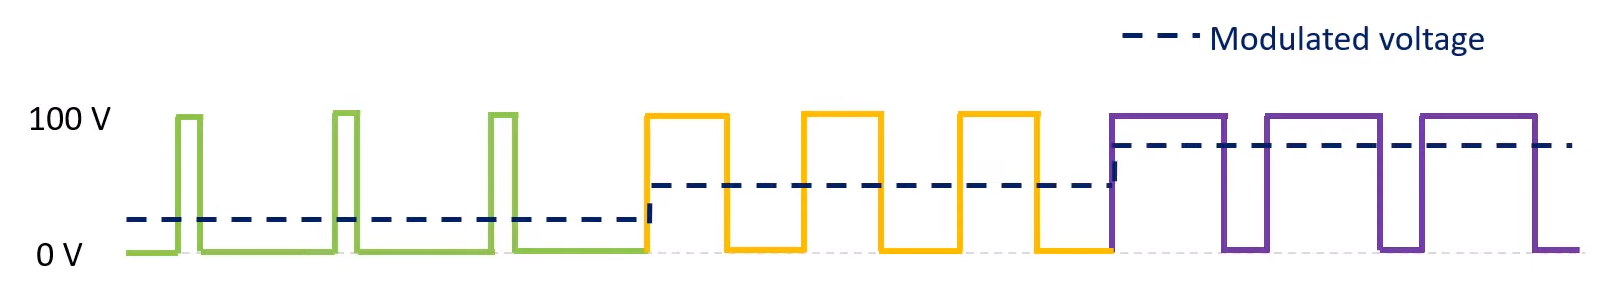
\includegraphics[width=13cm]{imagens/PWM.png}
	\caption*{Fonte:\cite{matlabBLDC}.}
 \label{Modulação por largura de pulso utilizando uma fonte de 100V}
\end{figure}

\subsubsection{Outros Algoritmos de Controle}

Além do Controle Trapezoidal existem outras formas de controle que envolvem algorítimos mais complexos, como o Controle de Torque Vetorial e o Controle de Campo Orientado, ambos em malha fechada.

No controle de torque vetorial, o controlador de motor calcula a corrente que deve ser fornecida às bobinas do estator usando um modelo matemático do motor. O modelo matemático do motor descreve a relação entre a corrente nas bobinas do estator, o campo magnético do rotor e o torque produzido pelo motor. O controlador vetorial de torque do motor calcula o torque desejado e, em seguida, usa o modelo matemático do motor para calcular a corrente necessária para produzir o tal torque. Este controle é um método preciso e flexível que pode ser usado em uma variedade de aplicações. Ele é adequado para aplicações onde a exatidão de velocidade e torque é crítica

No controle de campo orientado, o controlador do motor calcula a corrente que deve ser fornecida às bobinas do estator usando a orientação do campo magnético do rotor. O controlador de motor usa um sensor para medir a orientação do campo magnético do rotor, sendo que o sensor envia um sinal para o controlador, o utiliza sinal para calcular a corrente necessária para manter o campo magnético do rotor na orientação desejada. O controle de campo orientado é um método preciso e eficiente que pode ser usado em aplicações de alta velocidade.

\pagebreak

\section{Vantagens e Desvantagens no uso de motores BLDC}
Os motores sem escovas, ou BLDC, apresentam diversas vantagens que contribuem para seu destaque em várias aplicações. O rendimento é uma característica proeminente, uma vez que convertem mais eficientemente a energia elétrica em torque quando comparados aos motores com escovas. Isso implica em uma demanda menor de energia para gerar a mesma quantidade de torque, resultando em um melhor desempenho global. A durabilidade é significativamente aprimorada, visto que a vida útil estendida desses motores está relacionada à ausência das escovas, componentes propensos a desgaste em motores convencionais.

Os motores de indução trifásicos (MIT) são concorrentes diretos dos motores BLDC, sendo que ambos são amplamente utilizados em diversas aplicações, cada uma com suas características distintas e vantagens específicas. Os motores de indução trifásicos são conhecidos pela sua confiabilidade, simplicidade de construção e custo relativamente baixo, quando comparado aos BLDC, utilizando os princípios da indução eletromagnética para gerar o torque e velocidade necessários para a aplicação. Embora tenham menor custo de produção quando comparados com os motores BLDC e podem ser controlados utilizando os mesmos protocolos, os MITs tendem a ter uma densidade de potência e torque menor em comparação com os motores BLDC, principalmente em baixas velocidades, o que pode ser uma consideração importante em aplicações que requerem alta potência em um espaço limitado. No entanto, os MITs apresentam melhor rendimento em operações de baixo torque, o que pode ser relevante em aplicações de mobilidade, como em veículos elétricos.

Os motores BLDC são conhecidos por seu rendimento energético superior, controle preciso de velocidade e torque, além de uma vida útil mais longa devido à ausência de escovas mecânicas \cite{gieras2009permanent}. Embora os BLDCs tenham um custo inicial mais elevado em comparação com os MITs, eles oferecem uma operação mais eficiente, especialmente em condições de carga variável e velocidade ajustável.

Em resumo, os motores sem escovas oferecem um conjunto de vantagens notáveis, incluindo rendimento aprimorado, operação mais silenciosa, maior durabilidade e menor necessidade de manutenção. Contudo, esses benefícios vêm com um custo inicial mais elevado e a exigência de um controlador de velocidade, o que pode tornar sua implementação menos acessível em certos contextos. A escolha entre motores com escovas e sem escovas dependerá das prioridades específicas de uma aplicação, considerando tanto os benefícios quanto as limitações de cada tecnologia.

\pagebreak

\section{Aplicações}
Os motores BLDC são amplamente utilizados em diversas aplicações devido às suas características únicas, como elevado rendimento, alta densidade de potência, baixo ruído, baixa manutenção e longa vida útil. Esses motores são preferidos em aplicações que necessitam de controle preciso de torque com oscilações inferiores em comparação com outros motores.

Uma das principais aplicações dos motores BLDC é em veículos elétricos, como carros, motocicletas, bicicletas e \textit{scooters} \cite{chau2007emerging}. Com o aumento da demanda por veículos elétricos, espera-se que os motores com tecnologia derivada do BLDC desempenhem um papel vital na indústria automotiva. Esses motores são usados para acionar o sistema de propulsão do veículo, fornecendo torque e potência para as rodas. Eles são preferidos em veículos elétricos devido à seu alta rendimento, baixo ruído e baixa manutenção. Essas motores são usados em aplicações que exigem alta precisão, controle de velocidade e torque, e baixo ruído.

\chapter{Objetivos}
Estudar o princípio de funcionamento de um controlador de motores Brushless, tornando possível o projeto e desenvolvimento de um protótipo que possa oferecer uma operação suave e precisa em diferentes cenários de aplicação.

\chapter{Metodologia}
O desenvolvimento do ESC será realizado em três etapas principais. A primeira conta com uma simulação computacional do sistema para entender a transformação da energia elétrica e a coordenação dos chaveamentos, analisando o controle de rotação e velocidade do motor. Em seguida, na fase de projeto, serão definidos os requisitos mínimos, escolhidos os componentes eletrônicos e desenvolvido o circuito, incluindo controle de tensão, corrente com sinais PWM e proteções. Por último, na prototipagem, o controlador será montado em uma PCB, programado e testado em laboratório para garantir o funcionamento e identificar melhorias.

\section{Simulação}
Para o desenvolvimento de um ESC, primeiramente, apresenta-se a simulação do sistema via software, permitindo assim um maior entendimento de cada etapa de transformação da energia elétrica, como a metodologia adotada para coordenação dos chaveamentos, sem as limitações físicas impostas na implementação do circuito real. A simulação gera uma análise teórica funcional sobre o controle de sentido de rotação e velocidade imposta ao motor.

\pagebreak

\section{Projeto}
Para a elaboração do projeto físico é necessário o levantamento dos requisitos mínimos que o projeto deve atender, como a categoria de motores que deve atender e sua fonte de alimentação. Em seguida será necessária a seleção dos componentes eletrônicos (drivers, transistores, bateria, entre outros), considerando características como um controlador adequado, tensão de operação, frequência de comutação, corrente máxima suportada e possíveis proteções para o sistema.

O projeto do circuito começa pelo controle de tensão, em seguida será projetado o controle de corrente fornecida às bobinas do motor através de sinais de PWM para controle de velocidade e sentido de rotação, ou seja o drive para motor BLDC e recursos adicionais como proteções térmicas ou de sobrecarga.

\section{Prototipagem}
Com o fim do projeto do circuito inicia-se a implementação do controlador em uma placa de circuito impresso (PCB) por meio de um software de design eletrônico. Com a montagem dos componentes na PCB, será necessária a programação do microcontrolador implementado a lógica de chaveamento e outras funções. Também serão realizados teste de funcionamento em laboratório para garantir o funcionamento correto do circuito e levantar possíveis melhorias ou correções. Após as devidas correções serão realizados testes de desempenho afim de verificar se o projeto atende os requisitos estabelecidos de potência e tempo de resposta.

Todas as partes relevantes durante o trabalho de graduação serão documentadas através da redação do relatório acadêmico e apresentação para a defesa do trabalho de graduação.

%% Por enquanto não sei onde colocar essa parte, mas será útil para estudo e será aproveitado
\newpage

\section{Escolha de Componentes}
A escolha dos outros itens do projeto foi baseada em um motor brushless comercial e a partir de suas especificações os outros componentes foram sendo escolhidos com características compatíveis ao motor ou que atendessem as necessidades do projeto.

\subsection{Motor}
O motor BLDC Turnigy XK3674-$2200KV$ é um modelo comercial projetado principalmente para Automodelismo, sendo do tipo Inrunner possui quatro polos, $2200KV$, Tensão Nominal de $25,2V$, Corrente Nominal de $70A$ e sendo capaz de produzir até $1750W$ de potência. A velocidade e torque a vazio do motor, como já vistos nos segmentos \ref{KV} \ref{KT}, é de $55440 RPM$ e $X Nm$, desconsiderando efeitos dissipativos, como o atrito.

\begin{figure}[h]
	\centering
	\caption{Motor Brushless Turnigy XK3674-$2200KV$.}
	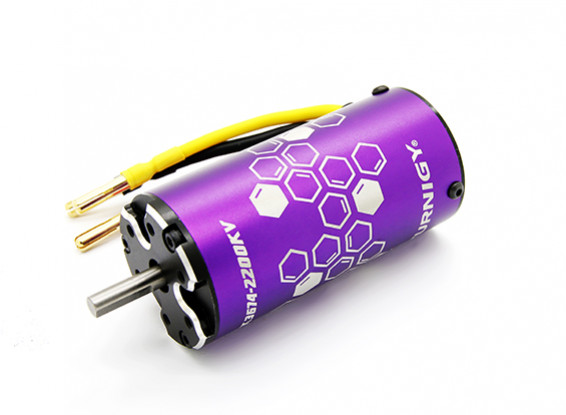
\includegraphics[width=8cm]{imagens/Turnigy XK3674-2200KV.jpg}
	\caption*{Fonte:\cite{turnigyMotor}.}
 \label{Motor Brushless Turnigy XK3674-2200KV}
\end{figure}

\subsection{Alimentação do Circuito}
Em uma aplicação móvel para o ESC devemos fazer uso de baterias como a única fonte de potência para alimentar todo o sistema. Os valores nominais de tensão e corrente do motor a devem ser supridos pela bateria, por volta de $26V$ e $70A$, mas considerando momentos de pico de corrente como por exemplo, uma situação de rotor travado ou de inversão de sentido de rotação é usada uma margem de segurança arbitrária de $30\%$, logo a bateria deve ser capaz de entregar $91A$ de corrente na descarga, um valor considerado alto para baterias.

Baterias tem três principais características:
\begin{itemize}
\item Tensão Nominal: Diferença de potencial fornecida pela bateria, normalmente é apresentado em em $S$, sendo esse o número de células que a bateira possui, sendo cada célula em média de $3,7V$, logo uma bateria de $7S$ tem uma tensão nominal de $25,9V$; 
\item Capacidade: Indica a quantidade de carga que a bateria pode fornecer antes de ser descarregada completamente, Normalmente é medida em miliampere-horas ($mAh$) ou ampere-horas ($Ah$);
\item Taxa de Descarga (ou \textit{C-rate}): Define a quantidade de corrente que a bateria pode fornecer sem danificar-se, é expressa em múltiplos de $C$.
\end{itemize}

Atualmente, a tecnologia de bateria com a maior taxa de descarga disponível comercialmente é a bateria de lítio de polímero (LiPo), podendo atingir taxas de descarga muito altas, que podem ultrapassar a $100C$, dependendo da aplicação e do design. Para calcular a corrente que tais baterias conseguem fornecer podemos aplicar a equação \ref{Corrente de uma bateria LiPo}, desconsiderando efeitos dissipativos ou a variação de tensão nominal que varia de acordo com o nível de carga da bateria, vale ressaltar que a capacidade da bateria deve estar em $Ah$.

\begin{equation}
I = C-rate * Capacidade
\label{Corrente de uma bateria LiPo}
\end{equation}

Uma bateria comercial que atende as especificações do projeto é o modelo Turnigy Graphene Panther $1300mAh$ $6S$ $75C$, capaz de fornecer por volta de $97,5A$, superior a margem de segurança estabelecida. Vale ressaltar que a baterias entrega de tensão nominal $22,2V$, inferior a tensão nominal o que para motores BLDC não é um problema, resultando apenas na redução da  sua velocidade nominal de $55440 RPM$ para $48840RPM$ a vazio, uma redução de aproximadamente $12\%$. 

\begin{figure}[h]
	\centering
	\caption{Turnigy Graphene Panther $1300mAh$ $6S$ $75C$.}
	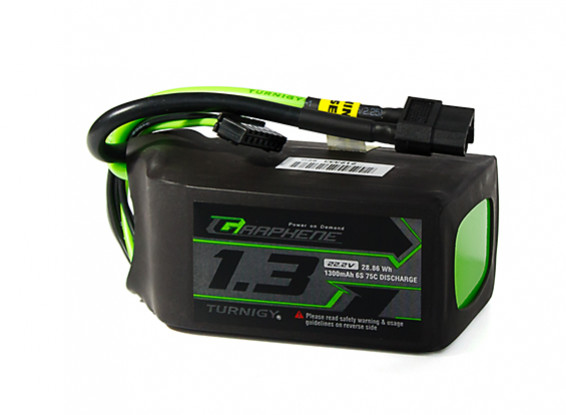
\includegraphics[width=9cm]{imagens/Turnigy Graphene Panther 1300mAh 6S 75C.jpg}
	\caption*{Fonte:\cite{turnigyBattery}.}
 \label{Turnigy Graphene Panther 1300mAh 6S 75C}
\end{figure}

\subsection{Microcontrolador}
Responsável por interpretar comando de entrada do usuário e gerar o acionamento correto da eletrônica para que assim o motor atue conforme o esperado pelo usuário. Para essa aplicação, foi selecionado ESP32-DevKit C, um microcontrolador de baixo custo e de código aberto,  utilizando o como principal elemento o módulo ESP32-WROOM-32 que opera entre $3V$ e $3,6V$ \cite{esp32-wroom-32Datasheet}, apresenta uma solução relevante para tais aplicações, especialmente em cenários que demandam controle em tempo real, conectividade IoT (\textit{Internet of Things}) ou arquiteturas de sistemas multifuncionais.

\begin{figure}[H]
	\centering
	\caption{Visão Geral do Microcontrolador ESP32-DevKit C.}
	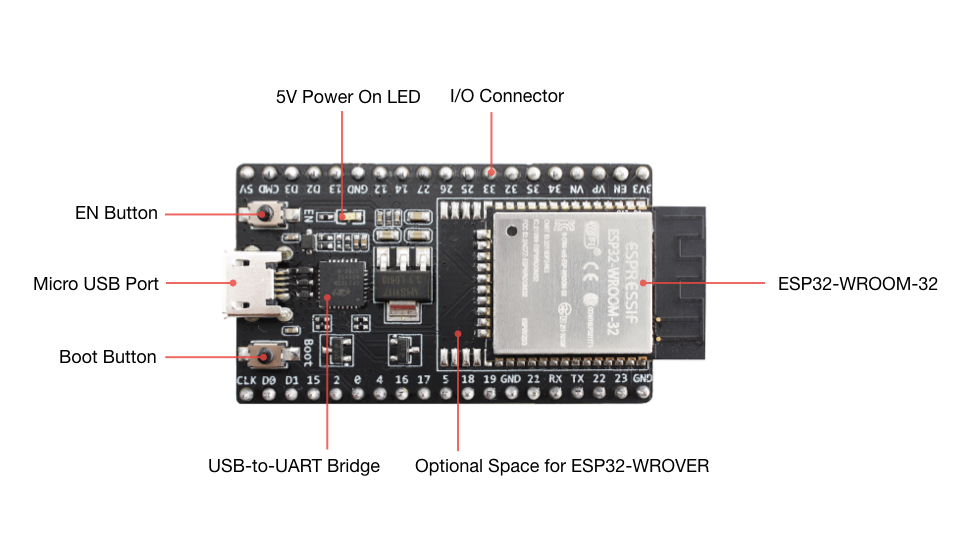
\includegraphics[width=10cm]{imagens/esp32-devkitc-v4-functional-overview.jpg}
	\caption*{Fonte:\cite{ESP32-DevKitCOverview}.}
 \label{esp32DevkitC}
\end{figure}

Por ser um projeto de código aberto existem diferentes implementações do mesmo módulo produzidas por vários fabricantes, a grande maioria delas possui as mesmas funcionalidades principais e variando tamanho da placa, outros módulos já implementados ou até mesmo reguladores de tensão permitindo a alimentação de $4,5V$ a $9V$ como é o caso do fornecido pela Robocore \cite{esp32DevkitV1}. No caso da ESP32-DevKit C, que será utilizado como base, é possível fornecer energia a mesma de três formas: Micro USB, $5V$ ou $3.3V$

Capaz de operar em velocidades de clock de até $240 MHz$, permitindo a execução paralela de tarefas, característica crítica para sistemas ESC que exigem simultaneidade entre o controle do motor (geração de sinais de modulação por largura de pulso (PWM)) e processos secundários, como aquisição de dados de sensores ou protocolos de comunicação. A resolução de 16 bits de até seis PWM de até 40 MHz no microcontrolador \cite{esp32-technical-reference-manual} amplia a precisão na comutação do motor, suportando frequências ajustáveis de até $40 MHz$, essenciais para minimizar a ondulação de torque em sistemas BLDC.

A integração de Wi-Fi e Bluetooth Low Energy (BLE) na arquitetura do ESP32 atende a demandas emergentes por sistemas de controle de motor habilitados para IoT. Essa capacidade viabiliza monitoramento remoto, atualizações de firmware over-the-air (OTA) e integração com plataformas baseadas em nuvem, aspectos cada vez mais prioritários em automação industrial e robótica inteligente. Adicionalmente, a extensa interface GPIO (Figura \ref{esp32DevkitCPinLayout}) do microcontrolador suporta componentes periféricos, como sensores de efeito Hall, codificadores incrementais, conversores analógico-digitais (ADCs) e acionamento de drivers, permitindo configurações de controle em malha fechada ou abertas sem circuitos externos de condicionamento de sinal.

\begin{figure}[H]
	\centering
	\caption{Pinagem do Microcontrolador ESP32-DevKit C.}
	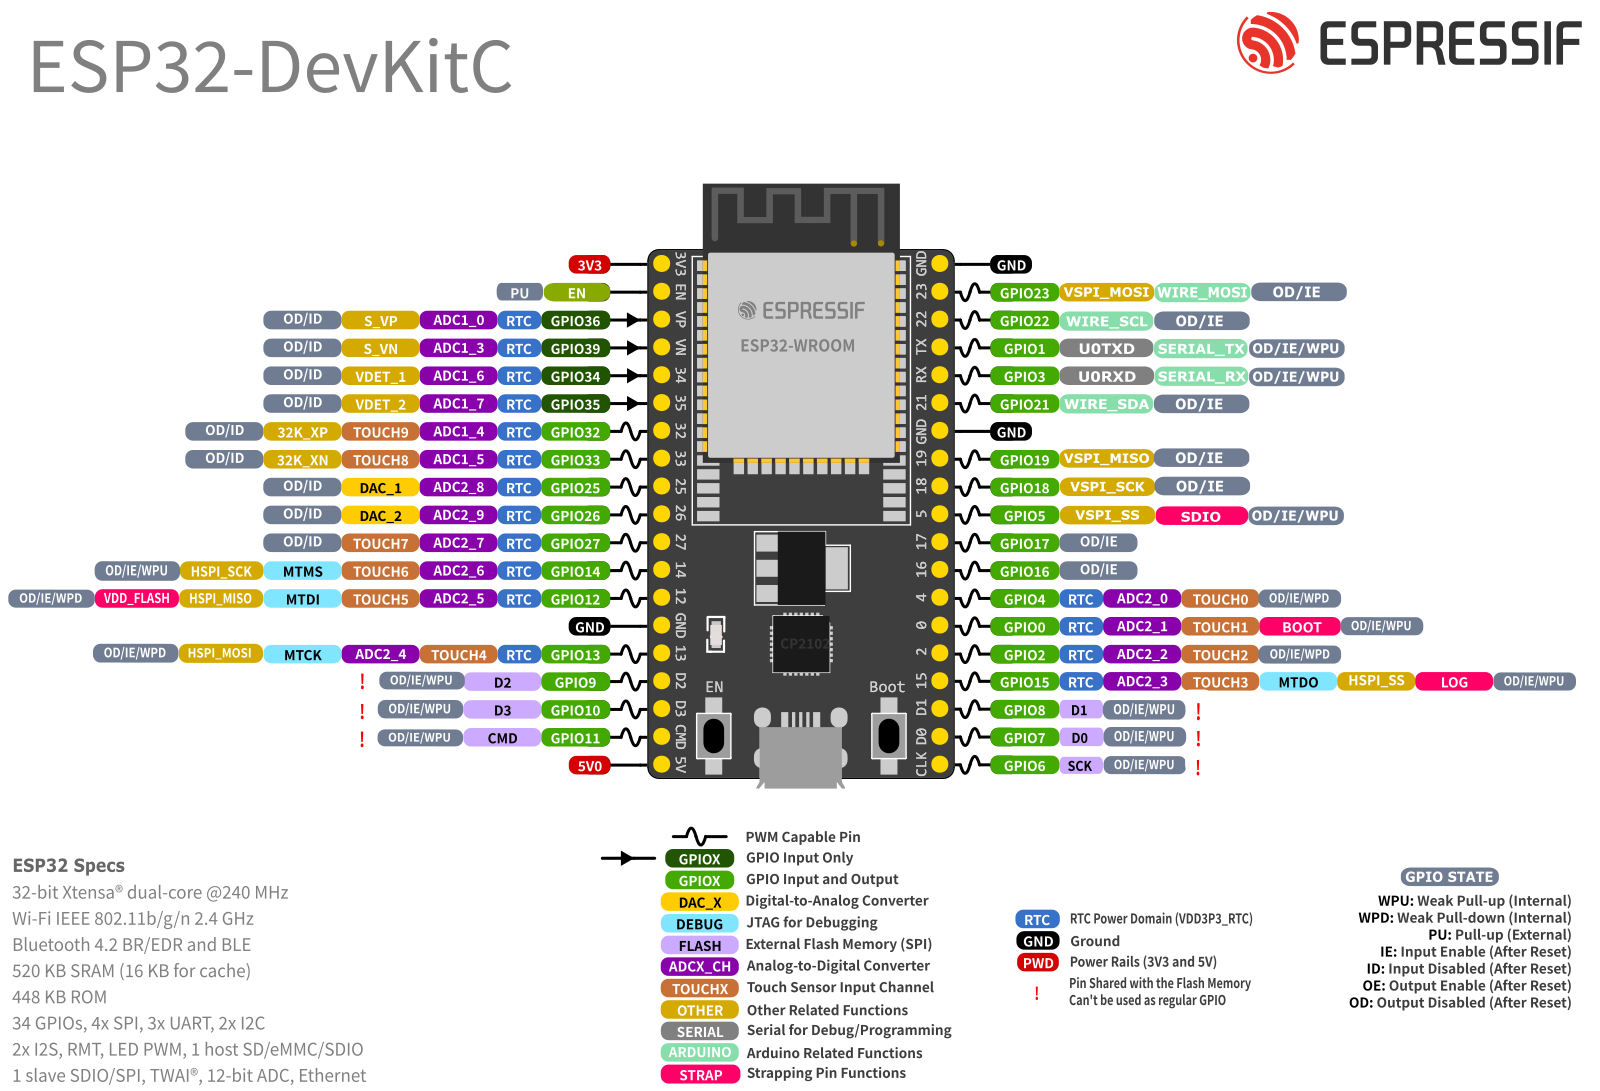
\includegraphics[width=16cm]{imagens/esp32_devkitC_v4_pinlayout.png}
	\caption*{Fonte:\cite{ESP32-DevKitCOverview}.}
 \label{esp32DevkitCPinLayout}
\end{figure}

A flexibilidade de software reforça ainda mais a viabilidade do ESP32. A compatibilidade com os ecossistemas Arduino e PlatformIO acelera o desenvolvimento por meio de bibliotecas pré-validadas para controle de motores. Por exemplo, um núcleo do processador pode ser dedicado a algoritmos de controle orientado a campo (field-oriented control, FOC), enquanto o segundo gerencia comunicação sem fio ou interfaces de usuário, reduzindo riscos de latência inerentes a arquiteturas single-core.

Apesar dessas vantagens, algumas limitações merecem consideração. Os níveis lógicos de $3,3V$ do ESP32 podem exigir circuitos de conversão de nível ao interagir com drivers de motor ou sensores de $5V$, aumentando a complexidade do projeto. Além disso, embora seu poder computacional seja vantajoso para sistemas multifuncionais, aplicações ESC mais simples sem requisitos de IoT podem incorrer em custo ou consumo energético desnecessários em comparação com MCUs dedicadas ao controle de motores (série STM32F3).

\subsection{Alimentação do Microcontrolador}
Existem duas abordagens possíveis para a alimentação do microcontrolador, utilizar uma segunda bateria de $5V$ ou reduzir o nível de tensão da bateria principal, apesar de ser a solução mais fácil pode impactar economia de peso e volume, fatores determinantes na autonomia e desempenho de sistemas móveis. Além disso, a manutenção e a operação do sistema tornam-se mais complexa, pois haverão duas fonte de alimentação para serem monitoradas e recarregadas. Para otimizar o sistema é possível elaborar um circuito BEC (\textit{Battery Elimination Circuit}) que reduz, para um valor compatível com o  microcontrolador, a tensão fornecida pela a bateria. Nessa aplicação é necessário reduzir a tensão de $30V$ para $5V$.

Dentre as topologias disponíveis, destacam-se os conversores buck (step-down) e os conversores isolados do tipo flyback. O conversor chaveado Buck é amplamente utilizada para a redução de tensão, operando com elevada eficiência (tipicamente superior a $85\%$) \cite{TIBuckCalculation}, mesmo sob variação da carga ou da tensão de entrada, caso seja implementado com circuito de retroalimentação. Sua estrutura básica é composta por um interruptor (geralmente um MOSFET), um diodo, um indutor e um capacitor de filtro. Diferentemente dos reguladores lineares, o Buck dissipa pouca energia em forma de calor, o que o torna ideal para aplicações com restrições térmicas e de consumo energético. Além disso, sua implementação é mais simples e compacta em relação a conversores Flyback, os quais requerem transformadores e circuitos de controle mais complexos, além de maiores dimensões físicas.

Em aplicações onde não há necessidade de isolamento galvânico entre a bateria e o circuito lógico, o conversor Buck é a solução preferencial. No projeto será aplicado o módulo comercial de baixo custo LM2596, um conversor buck de $150kHz$ e $3A$ de corrente de saída e tensão de saída ajustável que nesse caso será $5V$, capaz de receber até $40V$ de tensão de entrada, mais que o suficiente para essa implementação \cite{LM2596}.

\section{Lógica de Chaveamento}
\section{Cálculo de Componentes}

% --- ELEMENTOS PÓS-TEXTUAIS ---
\postextual
\printbibliography

\end{document}